
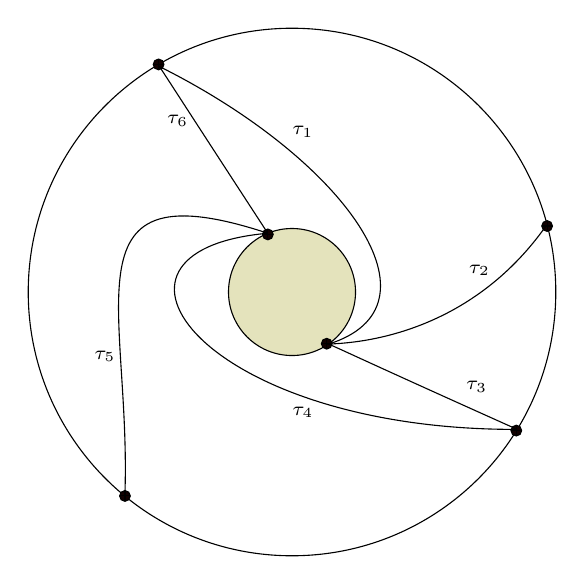
\begin{tikzpicture}[x=0.75pt,y=0.75pt,yscale=-1,xscale=1, scale = 0.9]
%uncomment if require: \path (0,458); %set diagram left start at 0, and has height of 458

%Shape: Circle [id:dp011167431945667827] 
\draw   (11,248.38) .. controls (11,170.39) and (74.22,107.17) .. (152.21,107.17) .. controls (230.2,107.17) and (293.42,170.39) .. (293.42,248.38) .. controls (293.42,326.36) and (230.2,389.58) .. (152.21,389.58) .. controls (74.22,389.58) and (11,326.36) .. (11,248.38) -- cycle ;
%Shape: Circle [id:dp7048127758853319] 
\draw  [fill={rgb, 255:red, 228; green, 227; blue, 188 }  ,fill opacity=1 ] (118.21,248.38) .. controls (118.21,229.6) and (133.43,214.38) .. (152.21,214.38) .. controls (170.99,214.38) and (186.21,229.6) .. (186.21,248.38) .. controls (186.21,267.15) and (170.99,282.38) .. (152.21,282.38) .. controls (133.43,282.38) and (118.21,267.15) .. (118.21,248.38) -- cycle ;
\draw  [fill={rgb, 255:red, 19; green, 1; blue, 1 }  ,fill opacity=1 ] (77.92,126.55) .. controls (77.92,124.97) and (79.2,123.69) .. (80.78,123.69) .. controls (82.36,123.69) and (83.64,124.97) .. (83.64,126.55) .. controls (83.64,128.13) and (82.36,129.42) .. (80.78,129.42) .. controls (79.2,129.42) and (77.92,128.13) .. (77.92,126.55) -- cycle ; \draw   (77.92,126.55) -- (83.64,126.55) ; \draw   (80.78,123.69) -- (80.78,129.42) ;
\draw  [fill={rgb, 255:red, 19; green, 1; blue, 1 }  ,fill opacity=1 ] (59.92,357.55) .. controls (59.92,355.97) and (61.2,354.69) .. (62.78,354.69) .. controls (64.36,354.69) and (65.64,355.97) .. (65.64,357.55) .. controls (65.64,359.13) and (64.36,360.42) .. (62.78,360.42) .. controls (61.2,360.42) and (59.92,359.13) .. (59.92,357.55) -- cycle ; \draw   (59.92,357.55) -- (65.64,357.55) ; \draw   (62.78,354.69) -- (62.78,360.42) ;
\draw  [fill={rgb, 255:red, 19; green, 1; blue, 1 }  ,fill opacity=1 ] (136.42,217.55) .. controls (136.42,215.97) and (137.7,214.69) .. (139.28,214.69) .. controls (140.86,214.69) and (142.14,215.97) .. (142.14,217.55) .. controls (142.14,219.13) and (140.86,220.42) .. (139.28,220.42) .. controls (137.7,220.42) and (136.42,219.13) .. (136.42,217.55) -- cycle ; \draw   (136.42,217.55) -- (142.14,217.55) ; \draw   (139.28,214.69) -- (139.28,220.42) ;
\draw  [fill={rgb, 255:red, 19; green, 1; blue, 1 }  ,fill opacity=1 ] (167.92,276.05) .. controls (167.92,274.47) and (169.2,273.19) .. (170.78,273.19) .. controls (172.36,273.19) and (173.64,274.47) .. (173.64,276.05) .. controls (173.64,277.63) and (172.36,278.92) .. (170.78,278.92) .. controls (169.2,278.92) and (167.92,277.63) .. (167.92,276.05) -- cycle ; \draw   (167.92,276.05) -- (173.64,276.05) ; \draw   (170.78,273.19) -- (170.78,278.92) ;
\draw  [fill={rgb, 255:red, 19; green, 1; blue, 1 }  ,fill opacity=1 ] (269.42,322.55) .. controls (269.42,320.97) and (270.7,319.69) .. (272.28,319.69) .. controls (273.86,319.69) and (275.14,320.97) .. (275.14,322.55) .. controls (275.14,324.13) and (273.86,325.42) .. (272.28,325.42) .. controls (270.7,325.42) and (269.42,324.13) .. (269.42,322.55) -- cycle ; \draw   (269.42,322.55) -- (275.14,322.55) ; \draw   (272.28,319.69) -- (272.28,325.42) ;
\draw  [fill={rgb, 255:red, 19; green, 1; blue, 1 }  ,fill opacity=1 ] (285.92,213.05) .. controls (285.92,211.47) and (287.2,210.19) .. (288.78,210.19) .. controls (290.36,210.19) and (291.64,211.47) .. (291.64,213.05) .. controls (291.64,214.63) and (290.36,215.92) .. (288.78,215.92) .. controls (287.2,215.92) and (285.92,214.63) .. (285.92,213.05) -- cycle ; \draw   (285.92,213.05) -- (291.64,213.05) ; \draw   (288.78,210.19) -- (288.78,215.92) ;
%Curve Lines [id:da8637706579523565] 
\draw    (80.75,127.42) .. controls (80.75,126.42) and (81.25,127.92) .. (139.25,216.92) ;
%Curve Lines [id:da8931038200838086] 
\draw    (80.75,127.42) .. controls (181.25,177.42) and (236.75,256.42) .. (171.25,276.42) ;
%Curve Lines [id:da4496396466165504] 
\draw    (171.25,276.42) .. controls (171.25,275.42) and (171.25,276.42) .. (272.75,321.92) ;
%Curve Lines [id:da8914629129152412] 
\draw    (171.25,276.42) .. controls (171.25,275.42) and (241.25,279.42) .. (288.25,212.92) ;
%Curve Lines [id:da9415141411706016] 
\draw    (139.25,216.92) .. controls (32.75,226.42) and (105.25,322.42) .. (272.75,321.92) ;
%Curve Lines [id:da7175871064348958] 
\draw    (139.25,216.92) .. controls (28.75,180.5) and (66.25,256.5) .. (62.75,357) ;

% Text Node
\draw (151,158.4) node [anchor=north west][inner sep=0.75pt]  [font=\scriptsize]  {$\tau _{1}$};
% Text Node
\draw (245.5,232.4) node [anchor=north west][inner sep=0.75pt]  [font=\scriptsize]  {$\tau _{2}$};
% Text Node
\draw (244,294.9) node [anchor=north west][inner sep=0.75pt]  [font=\scriptsize]  {$\tau _{3}$};
% Text Node
\draw (151,308.4) node [anchor=north west][inner sep=0.75pt]  [font=\scriptsize]  {$\tau _{4}$};
% Text Node
\draw (45,278.4) node [anchor=north west][inner sep=0.75pt]  [font=\scriptsize]  {$\tau _{5}$};
% Text Node
\draw (84,152.4) node [anchor=north west][inner sep=0.75pt]  [font=\scriptsize]  {$\tau _{6}$};

\end{tikzpicture}
\begin{tikzcd}
	& 2 &&& 3 \\
	\\
	1 &&&&& 4 \\
	\\
	& 6 &&& 5
	\arrow[from=1-2, to=3-1]
	\arrow[from=1-5, to=1-2]
	\arrow[from=1-5, to=3-6]
	\arrow[from=5-5, to=3-6]
	\arrow[from=5-2, to=5-5]
	\arrow[from=5-2, to=3-1]
\end{tikzcd}
